% VUT FIT MITAI
% MSZ 2021/2022
% Author: Vladimir Dusek
% Login: xdusek27

%%%%%%%%%%%%%%%%%%%%%%%%%%%%%%%%%%%%%%%%%%%%%%%%%%%%%%%%%%%%%%%%%%%%%%%%%%%%%%%%

% Path to figures
\graphicspath{{pds/smerovace/figures}}

%%%%%%%%%%%%%%%%%%%%%%%%%%%%%%%%%%%%%%%%%%%%%%%%%%%%%%%%%%%%%%%%%%%%%%%%%%%%%%%%

\chapter{PDS~--~Základní funkce směrovače, zpracování paketů ve směrovači, typy přepínání a architektur.}

%%%%%%%%%%%%%%%%%%%%%%%%%%%%%%%%%%%%%%%%%%%%%%%%%%%%%%%%%%%%%%%%%%%%%%%%%%%%%%%%

\section{Zdroje}

\begin{compactitem}
    \item \path{05-routing.pdf}
    \item \path{PDS_2021-03-12.mp4}
\end{compactitem}

%%%%%%%%%%%%%%%%%%%%%%%%%%%%%%%%%%%%%%%%%%%%%%%%%%%%%%%%%%%%%%%%%%%%%%%%%%%%%%%%

\section{Úvod a kontext}

% smerovaci tabulka
% prepinaci tabulka
% arp cache
% CAM tabulka
% route cache

\paragraph*{Fragmentace paketů} Uzel v síti (směrovač) dostane paket o velikosti $n$. Paket má přeposlat přes výstupní rozhraní do sítě, ve které je $MTU < n$. Aby paket mohl být odeslán, musí být rozdělen (fragmentován) na více menších paketů (fragmenty) a odeslán po částech. Na straně příjemce pak musí nastat opačný proces~--~defragmentace.

\paragraph*{MTU} MTU (\textit{Maximum Transmission Unit}) je největší velikost paketu, kterou lze v síti odeslat (přes výstupní rozhraní síťového prvku). Závisí na síťové kartě příslušného rozhraní.

%%%%%%%%%%%%%%%%%%%%%%%%%%%%%%%%%%%%%%%%%%%%%%%%%%%%%%%%%%%%%%%%%%%%%%%%%%%%%%%%

\section{Základní popis směrovače}

Směrovač je síťové zařízení, které předává datové pakety mezi počítačovými sítěmi. Základní charakteristika: \begin{compactitem}
    \item Pracuje s pakety (síťová vrstva, L3).
    \item Tvoří rozhraní mezi počítačovými sítěmi (provádí překlad NAT).
    \item Klasifikuje a filtruje pakety (firewall, ACL).
    \item Provádí fragmentaci a defragmentaci.
\end{compactitem}

\paragraph*{Činnost} \begin{compactenum}
    \item Vypouzdření paketu z L2 (odebrání L2 hlavičky) a kontrola jestli je v pořádku (pomocí kontrolního součtu).
    \item Vyhledání cesty kam se má paket směrovat a překlad adresy NAT (pomocí směrovací tabulky).
    \item Určení cílové MAC adresy na základě cílové IP adresy (pošle ARP dotaz).
    \item Určení výstupního rozhraní.
    \item Sestavení výsledného paketu podle výstupního rozhraní (zapouzdření do příslušné L2 technologie~--~přidání L2 hlavičky).
\end{compactenum}

\paragraph*{Co ovlivňuje propustnost} \begin{compactitem}
    \item Rozbalení paketu.
    \item Vyhledání směrovací cesty.
    \item Překlad NAT.
    \item Vyhledání cílové MAC adresy.
    \item Zabalení paketu do správné technologie.
\end{compactitem}

\paragraph*{Typy} \begin{compactitem}
    \item Páteřní směrovače~--~součástí pátečních sítí mezi ISP.
    \item Hraniční směrovače~--~mezi zákaznickými sítěmi a ISP.
    \item Podnikové směrovače~--~propojení koncových systému v podnikových (\textit{enterprise}) sítích.
    \item Domácí směrovače.
\end{compactitem}

%%%%%%%%%%%%%%%%%%%%%%%%%%%%%%%%%%%%%%%%%%%%%%%%%%%%%%%%%%%%%%%%%%%%%%%%%%%%%%%%

\section{Operace co směrovač vykonává}

Pakety mohou být určeny buď přímo pro směrovač (aktualizace směrovací cesty přes směrovací protokoly~--~aktualizace směrovací tabulky) a nebo jinému uzlu v síti. V takovém případě směrovač paket přeposílá dalším uzlům v síti.

\begin{compactitem}
    % \item Základní operace směrovače jsou definovány v RFC a musí je implementovat každý směrovač.
    \item \textbf{Směrování} (\textit{routing})~--~Určování cest paketů v prostředí počítačových sítí. Cílem je doručit paket adresátovi, pokud možno co nejefektivnější cestou. Směrování zajišťují nejen směrovače, ale i koncové stanice (při vysílání).
    \item \textbf{Přepínání} (\textit{forwarding, switching})~--~Přepnutí paketu ze vstupního rozhraní na výstupní (viz architektura přepínačů).
\end{compactitem}

\begin{figure}[H]
    \centering
    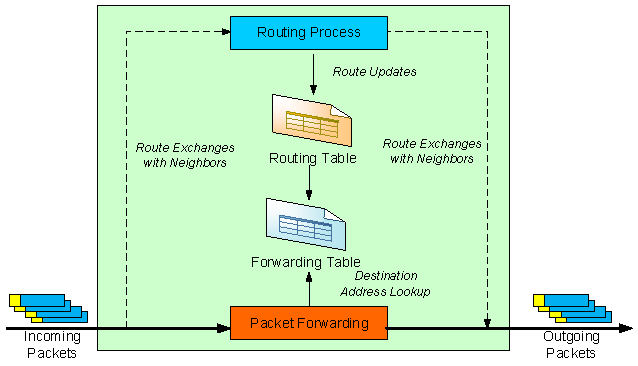
\includegraphics[width=1\linewidth]{smerovac_nakres.pdf}
    \caption{Základní činnost směrovače.}
\end{figure}

\paragraph*{Směrovací tabulka} Směrovací tabulka (\textit{routing table}) obsahuje informace nutné a dostačující pro směrování (\path{ip prefix}~--~IP prefix cílové sítě, \path{next hop}~--~IP adresa dalšího uzlu, \path{metrika}~--~cena cesty, počet hopů). Informace do ní se získavají pomocí směrovacích protokolů a nebo staticky (administrátor provede manuálně). Směrovací tabulku mají i koncové stanice (počítače), aby mohli posílat pakety do internetu.

\begin{figure}[H]
    \centering
    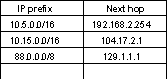
\includegraphics[width=0.4\linewidth]{smerovaci_tabulka.pdf}
    \caption{Příklad směrovací tabulky (bez metriky).}
\end{figure}

\paragraph*{Přepínací tabulka} Přepínací tabulka (FIB, \textit{forwarding information base}, \textit{forwarding table}) doplňuje směrovací tabulku o další informace, které jsou nutné pro sestavení cílového paketu (výstupní rozhraní, zdrojová MAC adresa, cílová MAC adresa). Informace do ní se získavají pomocí ARP protokolu a doplnění vlastních informací (\texttt{dst MAC address}).

\begin{figure}[H]
    \centering
    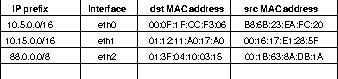
\includegraphics[width=0.9\linewidth]{prepinaci_tabulka.pdf}
    \caption{Příklad přepínací tabulky.}
\end{figure}

\paragraph*{Zpracování IP paketu (již vypouzdřeno z L2)} \begin{compactenum}
    \item Validace hlavičky L3 (formát, verze, délka).
    \item Kontrola hodnoty TTL a její dekrementace. Pokud je TLL 0, tak se paket zahodí a pošle ICMP zpráva.
    \item Přepočítání kontrolního součtu.
    \item Zpracování rozšířených voleb IP protokolu (timestamp, record route, strict source route).
    \item Vyhledání cesty (next-hop) na základě cílové adresy (lokální doručení, unicast, multicast). Pokud se nepodaří vyhledat cesta, tak se paket zahodí a pošle ICMP zpráva.
    \item Fragmentace a defragmentace IP paketů (pokud $MTU_{in} < MTU_{out}$).
    \item Zpracování zpráv ICMP a IGMP.
\end{compactenum}

\begin{figure}[H]
    \centering
    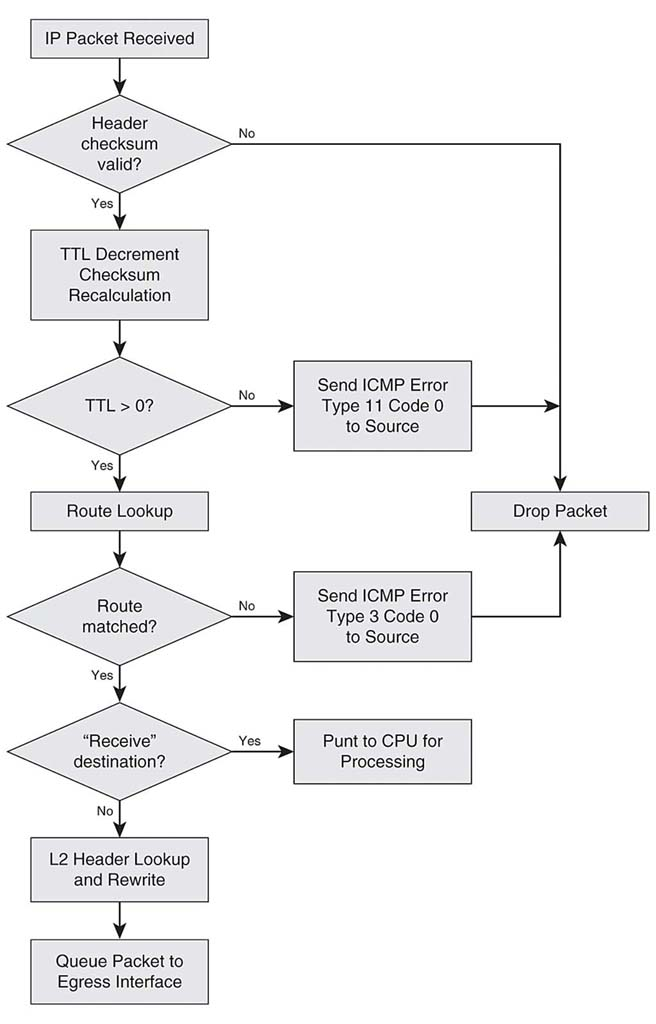
\includegraphics[width=0.75\linewidth]{cinnost_smerovace.png}
    \caption{Diagram zpracování paketu ve směrovači.}
\end{figure}

%%%%%%%%%%%%%%%%%%%%%%%%%%%%%%%%%%%%%%%%%%%%%%%%%%%%%%%%%%%%%%%%%%%%%%%%%%%%%%%%

\section{Architektura směrovače}

Rozdělíme na fyzické části (z hlediska hardware) a funkční části (z hlediska komponent co něco vykonávají).

\subsection{Fyzické části}

\begin{compactitem}
    \item Procesorová část (\textit{Router Processor Card})
    \item Přepínací logika (\textit{Switch Fabric Card})
    \item Síťové karty (\textit{Line Card})~--~každá má vstupní a výstupní rozhraní (\textit{Port Card})
\end{compactitem}

\begin{figure}[H]
    \centering
    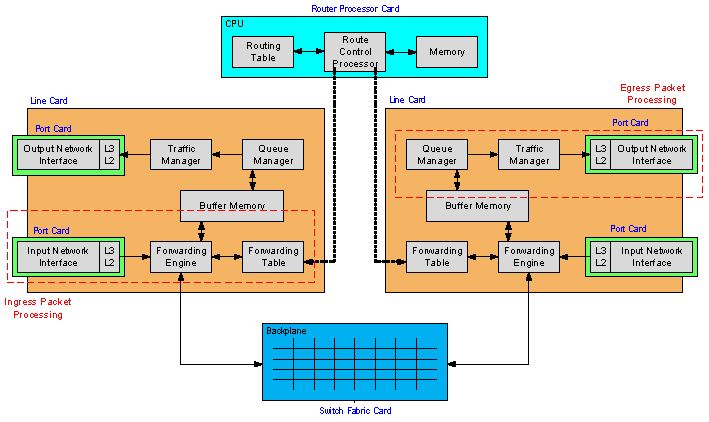
\includegraphics[width=1\linewidth]{architektura_fyzicke_casti.pdf}
    \caption{Fyzické části (procesory, paměti) směrovače.}
\end{figure}

\subsection{Funkční části}

\paragraph*{Procesorová část} procesor, paměť, směrovací tabulka \begin{compactitem}
    \item Implementuje směrování na obecném CPU
    \item Zpracovává směrovací informace: aktualizace, udržuje sousedství
    \item Obsluhuje směrovací tabulku
    \item Přenáší data do přepínací tabulky
    \item Zpracovává pakety, které nelze směrovat pomocí FIB
    \item Vytváří chybové zprávy ICMP
\end{compactitem}

\paragraph*{Přepínací logika} propojovací deska (\textit{Backplane})\begin{compactitem}
    \item Propojuje síťové rozhraní
    \item Vytváří sdílené (shared) či přepínané (switched) propojení
    \item Rychlost přepínání odpovídá přenosovému pásmu všech rozhraní
\end{compactitem}

\paragraph*{Síťové karty} \begin{compactitem}
    \item Vstupní/Výstupní síťové rozhraní (\textit{Input/Output Network Interface}) \begin{compactitem}
        \item Obsahuje více vstupních/výstupních portů
        \item Odstraní zapouzdření L2
        \item Předá hlavičku L3 přepínacímu modulu
        \item Uloží paket do paměti
        \item Zapouzdří odchozí pakety
    \end{compactitem}
    \item Řízení přepínání (\textit{Forwarding Engine}) \begin{compactitem}
        \item Dostane hlavičku L3 ze síťového rozhraní
        \item Určí výstupní rozhraní podle informace ve FIB
        \item Provádí klasifikace paketů pro podporu QoS na výstupu
    \end{compactitem}
    \item Správce front (\textit{Queue Manager}) \begin{compactitem}
        \item Ukládá pakety do vyrovnávací paměti, pokud je výstupní port obsazen
        \item Spravuje výstupní frontu $\rightarrow$ různé typy výstupních front
        \item Při zaplnění fronty vybírá a zahazuje pakety podle definované politiky
    \end{compactitem}
    \item Správce provozu (\textit{Traffic Manager}) \begin{compactitem}
        \item Prioritizuje a reguluje výstupní provoz podle požadavků QoS
        \item Omezuje či ořezává výstupní provoz (shaping, policing)
    \end{compactitem}
\end{compactitem}

\begin{figure}[H]
    \centering
    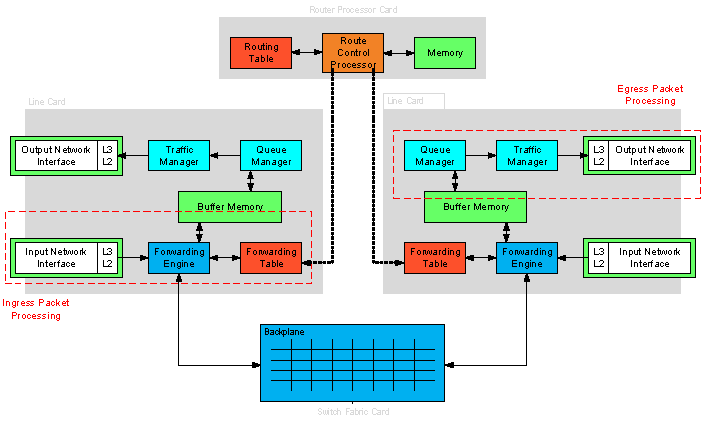
\includegraphics[width=1\linewidth]{architektura_funkci_casti.pdf}
    \caption{Funkční částí (procesy).}
\end{figure}

%%%%%%%%%%%%%%%%%%%%%%%%%%%%%%%%%%%%%%%%%%%%%%%%%%%%%%%%%%%%%%%%%%%%%%%%%%%%%%%%

\section{Zpracování paketu ve směrovači}

Směrovač můžeme rozdělit na dvě části: \begin{compactitem}
    \item \textit{Data Plane}~--~Specifický hardware pro zpracování paketu (rychlé zpracování)~--~ASIC.
    \item \textit{Control Plane}~--~Obecný procesor pro realizaci složitějších operací (pomalé zpracování).
    % todo (NAT, filtrovani pomoci ACL/firewall, fragmenta, defragmentace se obvykle musí zpracovávat tady)
\end{compactitem}

\begin{figure}[H]
    \centering
    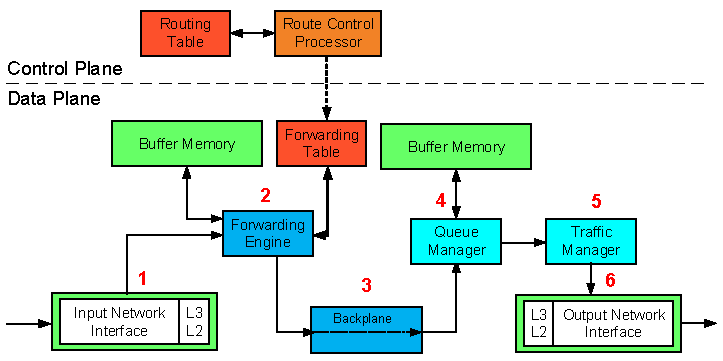
\includegraphics[width=1\linewidth]{control_plane_and_data_plane.pdf}
    \caption{Rozdělení přepínače na části \textit{Data Plane} a \textit{Control Plane} a zpracování rozděleno do 6. fází.}
\end{figure}

\paragraph*{Kontext paketu} Pomocná datová struktura, která reprezentuje paket uvnitř směrovače. Obsahuje vybrané informace z hlaviček. V rámci jednotlivých komponent směrovače se předává (pokud možno) tato struktura, pro větší efektivitu. Na počátku máme pouze částečný kontext, který se průběžně doplňuje. Na základě něho je pak sestaven výstupní paket.

\paragraph*{Fáze zpracování} Pokud některá z fází skončí neúspěšně, paket je zahozen. \begin{compactenum}
    \item Paket přijde na síťové rozhraní \begin{compactitem}
        \item Síťová karta zpracuje L2 rámec, zkontroluje FCS
        \item Vytvoří kontext paketu: vloží L2 zdrojovou a cílovou adresu
        \item Zpracování hlavičky L3: typ protokolu, kontrolní součet, TTL
        \item Doplnění kontextu o informace L3: IP adresy, typ protokolu, DSCP $+$ porty
    \end{compactitem}
    \item Zpracování v přepínacím modulu \begin{compactitem}
        \item Vyhledání cesty v přepínací tabulce: next hop $+$ výstupní rozhraní
        \item Doplnění dalších informací do kontextu paketu
        \item Paket uložen do vyrovnávací paměti $\rightarrow$ adresa vložena do kontextu
    \end{compactitem}
    \item Přeposlání kontextu propojovací deskou \begin{compactitem}
        \item Paket i kontext jsou přeneseny na výstupní rozhraní
    \end{compactitem}
    \item Zpracování správcem front \begin{compactitem}
        \item Podle priority v kontextu paketu je paket vložen do příslušné výstupní fronty
        \item Obsluha fronty probíhá podle daného plánovacího algoritmu
    \end{compactitem}
    \item Předání kontextu správci provozu \begin{compactitem}
        \item Kontrola omezení rychlosti (shaping) dle kontextu
        \item Překročení rychlost: zahození či zpomalení
    \end{compactitem}
    \item Výstupní síťové rozhraní \begin{compactitem}
        \item L3: aktualizace TTL, přepočítání kontrolního součtu
        \item L2: přidání hlavičky, výpočet CRC
        \item Odeslání paketu (zapsání na výstupní médium)
    \end{compactitem}
\end{compactenum}

\paragraph*{Plný kontext paketu} \begin{compactitem}
    \item Kontext doplněn o výstupní informace
    \item Základní deska přenese paket i kontext na
    \item výstupní rozhraní
    \item Kontext obsahuje adresu uložení paketu v paměti
    \item Zpracování paketu předáno správci front
\end{compactitem}

\begin{figure}[H]
    \centering
    \begin{subfigure}{.5\textwidth}
        \centering
        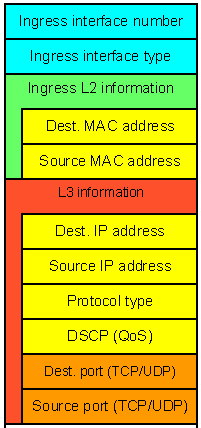
\includegraphics[width=.5\linewidth]{kontext_castecny.pdf}
        \caption{Kontext paketu~--~částečný.}
    \end{subfigure}%
    \begin{subfigure}{.5\textwidth}
        \centering
        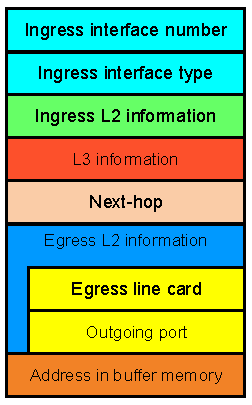
\includegraphics[width=.5\linewidth]{kontext_uplny.pdf}
        \caption{Kontext paketu~--~úplný.}
    \end{subfigure}
    \caption{Kontext paketu (\textit{ingress}~--~vstup, \textit{engress}~--~výstup.)}
\end{figure}

\noindent Paket může být zahozen i na výstupní kartě. Proč? \begin{compactitem}
    \item Vypršelo TTL
    \item Jsou plné fronty (politika RED, WRED)
    \item Filtrování na výstupu
\end{compactitem}

\noindent Paket může být zpracován dvěma způsoby: rychlou cestou (přes \textit{data plane}) a pomalou cestou (přes \textit{control plane}).

\paragraph*{Rychlá cesta} Paket je možné zpracovat pouze v hardwaru (\textit{data plane}). \begin{compactitem}
    \item Zpracování hlavičky IP (kontrola verze, délky paketu, snížení TTL, přepočítání kotrolního součtu)
    \item Přeposlání paketu ze vstupní na výstupní (lokální uložení, přeposlání na jeden port (unicast) či více portů (multicast))
    \item Klasifikace paketu na základě informací z hlavičky (optimalizované datové struktury pro rychlé uložení a vyhledání)
    \item Uložení do front, plánování (různé typy front, různé typy obsluhy)
\end{compactitem}

\paragraph*{Pomalá cesta} Paket je částečně zpracován v hardwaru, ale většina zpracování musí proběhnout softwarově (\textit{control plane}). Síťová karta nedokáže zpracovat paket sama a musí se využít centrální procesor. \begin{compactitem}
    \item Zpracování ARP (zjištění výstupní adresy L2: první paket, ostatní pakety)
    \item Fragmentace a defragmentace
    \item Generování zpráv ICMP
    \item Zpracování směrovacích informací
\end{compactitem}

\begin{figure}[H]
    \centering
    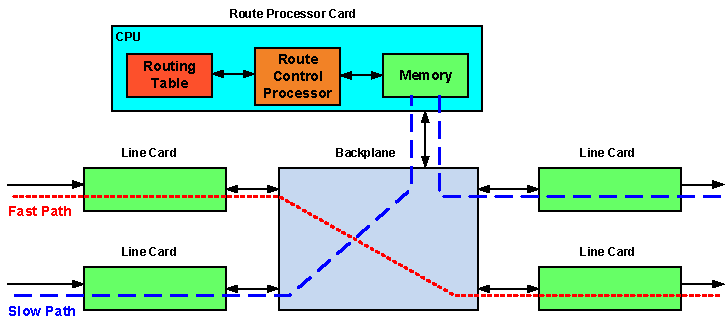
\includegraphics[width=1\linewidth]{rychla_a_pomala_cesta.pdf}
    \caption{Dva způsoby zpracování paketu ve směrovačí~--~pomalou cestou a rychlou cestou.}
\end{figure}

%%%%%%%%%%%%%%%%%%%%%%%%%%%%%%%%%%%%%%%%%%%%%%%%%%%%%%%%%%%%%%%%%%%%%%%%%%%%%%%%

\section{Typy přepínání paketů}

Přepínání paketů z jednoho rozhraní na druhé na základě směrovacích informací je jedna z nejdůležitějších funkcí směrovače. Proces přepínání paketů zahrnuje: \begin{compactitem}
    \item Zjištění, zda cíl cesty paketu je dosažitelný.
    \item Vyhledání nejbližšího uzlu na cestě (next-hop) a určení výstupního rozhraní.
    \item Vyhledání informací pro vytvoření L2 hlavičky paketu na výstupu.
\end{compactitem}

\subsection{Softwarové přepínání (\textit{Process Switching})}

\begin{compactitem}
    \item Přepínání pomocí centrálního procesoru s centrální pamětí. \begin{compactitem}
        \item Pomalé~--~přístup do paměti, obecný procesor (softwarové zpracování).
    \end{compactitem}
    \item Pro každý paket se hledá cesta ve směrovací tabulce a určuje se MAC adresa cíle.
    \item Směrovač využívá standardní mechanismus přepíná procesů v OS (přeřušení).
\end{compactitem}

\paragraph*{Fáze softwarového přepínání} \begin{compactenum}
    \item I/O procesor detekuje paket na vstupním médiu. Přenese ho do vstupního bufferu.
    \item I/O procesor vygeneruje přerušení. Během přerušení určí centrální procesor typ paketu a zkopíruje ho do centrální paměti.
    \item Centrální plánovač zjistí, že ve vstupní frontě je paket. Naplánuje jeho další zpracování procesem.
    \item Proces pro zpracování vyhledá ve směrovací tabulce další uzel (next hop) a výstupní rozhraní. V paměti ARP cache vyhledá MAC adresu dalšího uzlu.
    \item Přepíše L2 hlavičku paketu a umístí paket do výstupní fronty na výstupním portu.
    \item Paket vložen do fronty na výstupním portu.
    \item I/O procesor detekuje paket ve vysílací frontě. Zapíše ho na síťové médium.
\end{compactenum}

\begin{figure}[H]
    \centering
    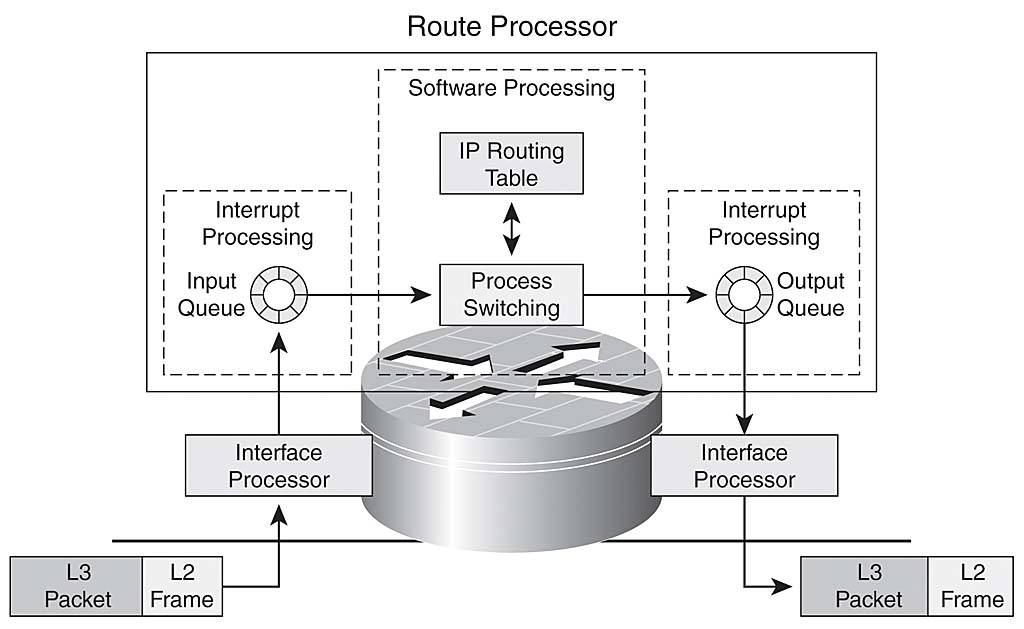
\includegraphics[width=1\linewidth]{softwarove_prepinani.png}
    \caption{Softwarové přepínání.}
\end{figure}

\paragraph*{Optimalizace} \begin{compactitem}
    \item Nejdéle trvá: na základě cíle vyhledávání informací ve směrovací tabulce, najdu next hop, najdu příslušný záznam v ARP tabulce
    \item Můžeme využít cache (která si bude pamatovat poslední záznamy.
\end{compactitem}

\subsection{Rychlé přepínání (\textit{Fast Switching})}

\begin{compactitem}
    \item Využívá vyrovnávací paměť \textit{route cache} s předpočítanou L2 hlavičkou.
    \item První paket toku se přepíná softwarově, další pakety toku jdou rychlou cestou.
    \item Při přepínání paketu je vložen do paměti \textit{route cache} nový záznam.
    \item Neexistuje synchronizace mezi směrovací tabulkou, ARP cache a \textit{route cache}.
    \item Záznam v \textit{route cache} se zneplatní při změně ARP cache či směrovací tabulky.
    \item Při zaplnění paměti nad určitou mez se začnou záznamy náhodně zahazovat.
\end{compactitem}

\begin{figure}[H]
    \centering
    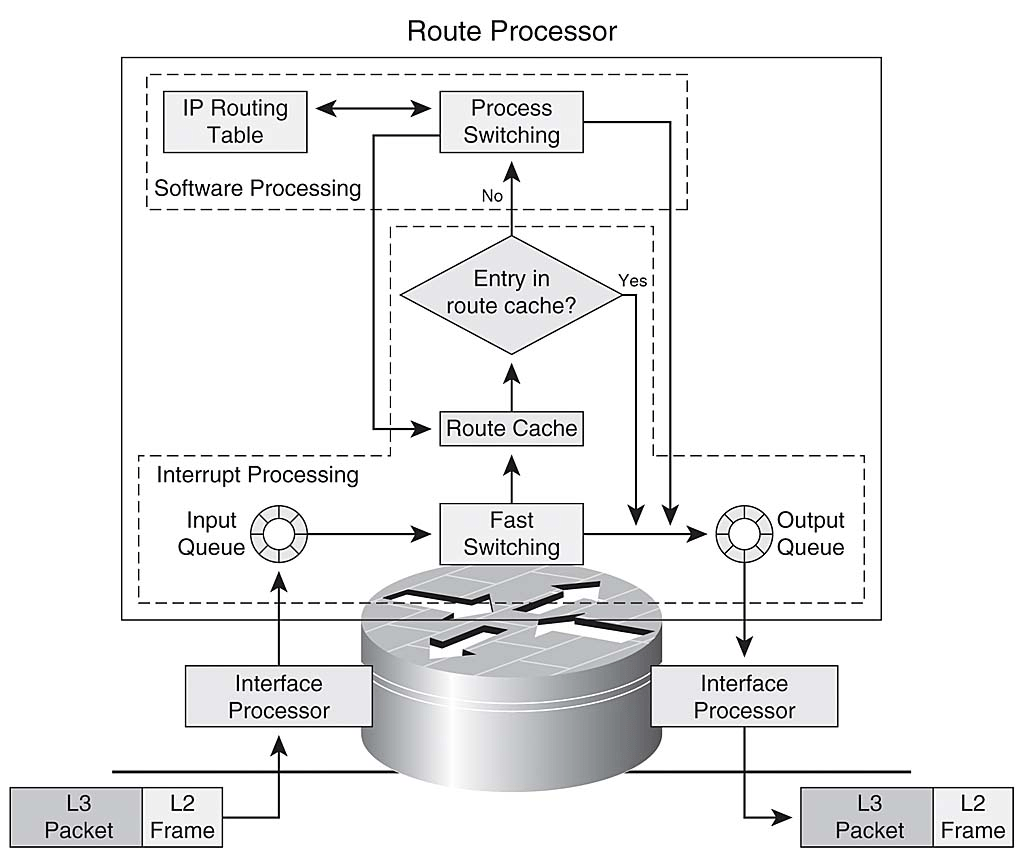
\includegraphics[width=1\linewidth]{rychle_prepinani.png}
    \caption{Rychlé přepínání.}
\end{figure}

\subsection{Expresní přepínání CEF (Cisco Express Forwarding)}

\todo{todo}

\begin{compactitem}
    \item Tabulka CEF se předpočítá na základě směrovací tabulky a tabulky sousedů ještě před příchodem paketu $\rightarrow$ nedochází k softwarovému přepínání.
    \item Oddělení směrovacích informací od L2 dat $\rightarrow$ nedochází ke stárnutí záznamů při expiraci záznamu v tabulce ARP.
    \item Změny ve směrovací tabulce či tabulce ARP se okamžitě propagují do tabulky CEF.
    \item ARP tabulka se synchronizuje se záznamy v tabulce sousedů.
\end{compactitem}

\begin{figure}[H]
    \centering
    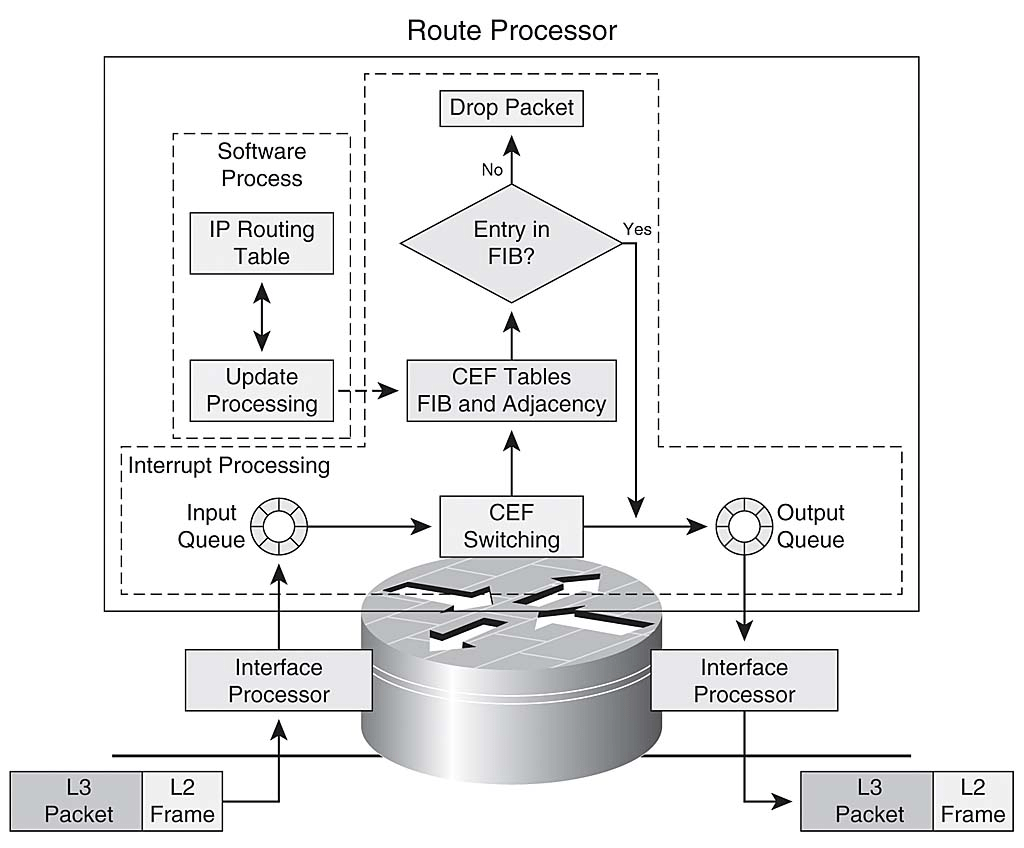
\includegraphics[width=1\linewidth]{expresni_prepinani.png}
    \caption{Expresní přepínání CEF.}
\end{figure}

%%%%%%%%%%%%%%%%%%%%%%%%%%%%%%%%%%%%%%%%%%%%%%%%%%%%%%%%%%%%%%%%%%%%%%%%%%%%%%%%

\section{Přehled architektur}

Architektury směrovačů rozdělmě podle způsobu přepínání paketů.

\subsection{Architektura se sdíleným procesorem}

\begin{compactitem}
    \item Využívá softwarové přepínání $\rightarrow$ každý paket zpracován na CPU.
    \item Cykly CPU rozděleny mezi přeposílání, směrování a další operace.
    \item Sdílená sběrnice i procesor $\Rightarrow$ levné, ale pomalé.
\end{compactitem}

\begin{figure}[H]
    \centering
    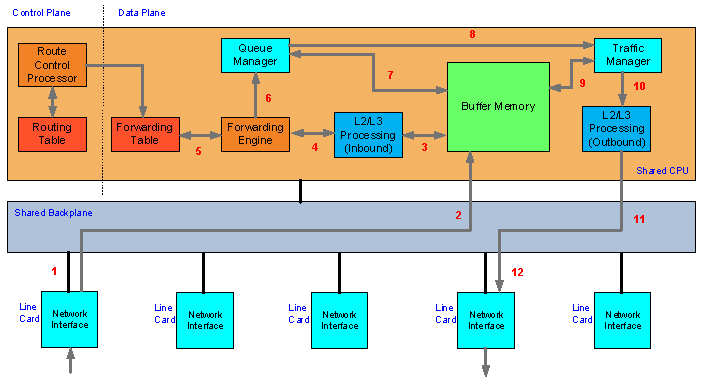
\includegraphics[width=0.95\linewidth]{architektura_se_sdilenym_procesorem.pdf}
    \caption{Architektura se sdíleným procesorem.}
\end{figure}

\subsection{Architektura se sdíleným procesorem a pamětí cache na kartě}

\begin{compactitem}
    \item Varianta s pamětí cache na kartě $\rightarrow$ synchronizace přepínacích tabulek.
    \item Síťová karta obsahuje FE pro zpracování hlaviček, paměť a přepínací tabulku.
    \item Rychlé přepínání (Fast Switching): první paket vs. další pakety.
\end{compactitem}

\begin{figure}[H]
    \centering
    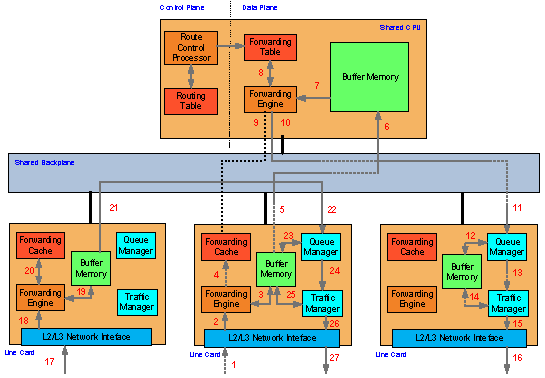
\includegraphics[width=0.95\linewidth]{architektura_se_sdilenym_procesorem_a_pameti_cache_na_karte.pdf}
    \caption{Architektura se sdíleným procesorem a pamětí cache na kartě.}
\end{figure}

\subsection{Architektura s nezávislými moduly FE}

\begin{compactitem}
    \item Přepínací moduly FE implementovány na speciálních kartách.
    \item Paralelní zpracování paketů, dvě sběrnice (sdílená a přepínaná).
\end{compactitem}

\begin{figure}[H]
    \centering
    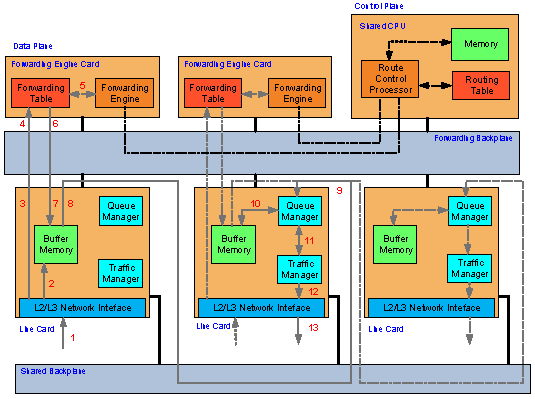
\includegraphics[width=0.95\linewidth]{architektura_s_nezavislymi_moduly_fe.pdf}
    \caption{Architektura s nezávislými moduly FE.}
\end{figure}

\subsection{Architektura s nezávislými moduly FE a přepínanou sběrnicí}

\begin{compactitem}
    \item Varianta s jednou přepínanou sběrnicí $\Rightarrow$ vyšší propustnost.
\end{compactitem}

\begin{figure}[H]
    \centering
    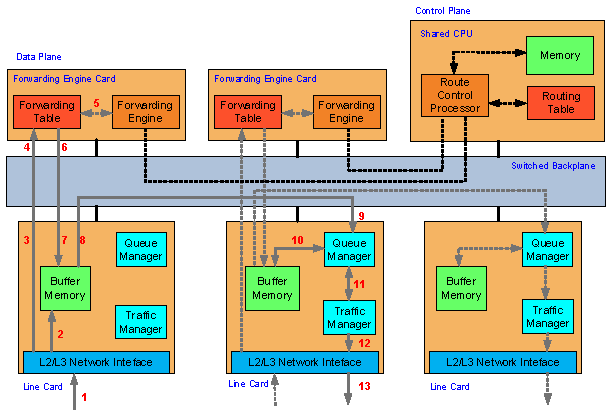
\includegraphics[width=0.95\linewidth]{architektura_s_nezavislymi_moduly_fe_a_prepinanou_sbernici.pdf}
    \caption{Architektura s nezávislými moduly FE a přepínanou sběrnicí.}
\end{figure}

\subsection{Distribuovaná architektura (Shared Nothing)}

\begin{compactitem}
    \item Veškeré zpracování paketu přeneseno do síťového modulu.
    \item Oddělení procesu směrování a přepínání $\rightarrow$ využití technologie CEF.
\end{compactitem}

\begin{figure}[H]
    \centering
    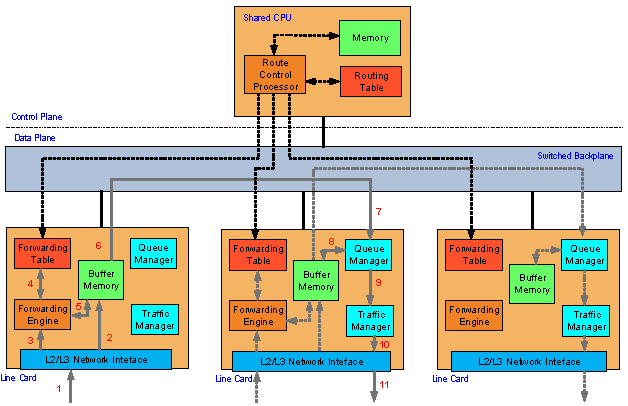
\includegraphics[width=0.95\linewidth]{architektura_distribuovana.pdf}
    \caption{Distribuovaná architektura (Shared Nothing).}
\end{figure}
